\documentclass[12pt,a4paper]{article}
\usepackage[utf8]{inputenc}

\usepackage{mathtools}
\usepackage{amsmath}
\usepackage{amssymb}
\usepackage{amsthm}
\usepackage{amssymb}
\usepackage{mathdots}
\usepackage[pdftex]{graphicx}
\usepackage{fancyhdr}
\usepackage[margin=1in]{geometry}
\usepackage{multicol}
\usepackage{bm}
\usepackage{listings}
\usepackage{xcolor}
\usepackage{pdfpages}
\usepackage{algpseudocode}
\usepackage{tikz}
\usepackage{enumitem}
\usepackage[T1]{fontenc}
\usepackage{inconsolata}
\usepackage{framed}
\usepackage{wasysym}
\usepackage[thinlines]{easytable}
\usepackage{hyperref}
\usepackage{minted}
\usemintedstyle{perldoc}
\hypersetup{
    colorlinks=true,
    linkcolor=blue,
    filecolor=magenta,      
    urlcolor=blue,
}
\definecolor{codegreen}{rgb}{0,0.6,0}
\definecolor{codegray}{rgb}{0.5,0.5,0.5}
\definecolor{codepurple}{rgb}{0.58,0,0.82}
\definecolor{backcolour}{rgb}{0.95,0.95,0.92}
\lstdefinestyle{mystyle}{
    backgroundcolor=\color{backcolour},   
    commentstyle=\color{codegreen},
    keywordstyle=\color{magenta},
    numberstyle=\tiny\color{codegray},
    stringstyle=\color{codepurple},
    basicstyle=\ttfamily,
    breakatwhitespace=false,         
    breaklines=true,                 
    captionpos=b,                    
    keepspaces=true,                 
    numbers=left,                    
    numbersep=5pt,                  
    showspaces=false,                
    showstringspaces=false,
    showtabs=false,                  
    tabsize=4
}
\lstset{style=mystyle}
\newcommand\numberthis{\addtocounter{equation}{1}\tag{\theequation}}
\newcommand{\rightqed}{
\begin{flushright}
$\blacksquare$
\end{flushright}
}
\newcommand{\solution}{\noindent\textbf{Solution:}\\}
\usepackage{graphics}
\usepackage{subfig}
\graphicspath{ {./images/} }

\title{CSCI 6690 Spectral Graph Theory Homework 4\\Isomorphisms and Drawings}
\author{Kushajveer Singh}
\date{}

\begin{document}
\maketitle

% Start problem 1
\subsection*{Problem 1}
\textit{
    Show that if $G$ and $G'$ are isomorphic, then $L_G = \Pi L_{G'}\Pi^T$. Show $L_G$ and $L_{G'}$ have same spectrum of eigenvalues.
}

\solution
(a) Given $G$ and $G'$ are isomorphic. So there must exist some function $f'$ that maps vertices of $G'$ to corresponding vertices in $G$ under some permutation $\pi^i$ i.e. 
\begin{equation}
f'(v_i') = v_{\pi'(i)} \label{eq:q_1_1}    
\end{equation}
where $v_i'$ is the vertex index of node $i'$ in $G'$ and $v_{\pi'(i)}$ is the corresponding vertex index of $v_i'$ in $G$.

Consider $\Pi L_{G'}$. We know multiplying by a permutation matrix on the left side of a matrix results in the permutation of rows of the matrix. So suppose $G^A$ is a graph with its graph laplacian given as $L_{G^A} = \Pi L_{G'}$. We observer that $G^A$ and $G'$ are isomorphic. This follows from the fact that $\Pi$ is just a permutation of rows, so the underlying graph structure remains same.

As $G^A$ and $G'$ are isomorphic, so there must exist some function $f^A$ that maps vertices of $G^A$ to corresponding vertices in $G'$ under some permutation $\pi^A$ i.e.
\begin{equation}
f^A(v_i^A) = v_{\pi^A(i)}' \label{eq:q_1_2}
\end{equation}

Now consider $L_{G^A}\Pi ^T$. We know multiplying by a permutation matrix on right side results in the permutation of the columns of the matrix. So suppose $G^B$ is a graph with its graph laplacian given as $L_{G^B} = L_{G^A}\Pi ^T$. We observe that $G^B$ and $G^A$ are isomorphic. This follows from the fact that $\Pi^T$ is just a permutation of columns, so the underlying graph structure remains same.

As $G^B$ and $G^A$ are isomorphic, so there must exist some function $f^B$ that maps vertices of $G^B$ to corresponding vertices in $G^A$ under some permutation $\pi^B$ i.e.
\begin{equation}
f^B(v_i^B) = v_{\pi^B(i)}^A \label{eq:q_1_3}
\end{equation}

Now,
\begin{align*}
    f^B(v_i^B) &= v_{\pi^B(i)}^A &\\
    f^A(f^B(v_i^B)) &= f^A(v_{\pi^B(i)}^A) &\textit{apply $f^A$ to both sides of equation}\\
    f^A(f^B(v_i^B)) &= v'_{\pi^A(\pi^B(i))} &\textit{from \eqref{eq:q_1_2}} \\
    f'(f^A(f^B(v_i^B))) &= f'(v'_{\pi^A(\pi^B(i))}) &\textit{apply $f'$ to both sides of equation}\\
    f'(f^A(f^B(v_i^B))) &= v_{\pi'(\pi^A(\pi^B(i)))} &\textit{from \eqref{eq:q_1_1}} \numberthis \label{eq:q_1_4}
\end{align*}

\eqref{eq:q_1_4}, we can compose $f'$, $f^A$, $f^B$ into a single function $f$ under some permutation $\pi$
\begin{equation}
    f(v_i^B) = v_{\pi(i)} \label{eq:q_1_5}
\end{equation}

$v_i^B$ is the node at index $i$ of graph $g^B$ whose laplacian is equal to $\Pi L_{G'}\Pi^T$. $f(v_i^B)$ gives us the corresponding index of node in graph $G$ under some permutation $\pi$.

We need to show there exists some permutation matrix for which $L_G$ and $\Pi L_{G'}\Pi^T$ are equal. From \eqref{eq:q_1_5}, we observer that $\pi(i) = i$ i.e. identity function solves this problem i.e. $\pi'(\pi^A(\pi^B(i))) = i$.
\rightqed

(b) In the last homework we proved, $(\Pi M\Pi^T)(\Pi v) = \lambda(\Pi v)$ where $v$ is the eigenvector of $M$ and $\lambda$ is the eigenvalue of $M$. Using this fact for $L_{G'}$, we get
\begin{align*}
    (\Pi L_{G'}\Pi^T)(\Pi v) &= \lambda(\Pi v) &\\
    L_G(\Pi v) &= \lambda(\Pi v) &\textit{as $L_G = \Pi L_{G'}\Pi^T$} \\
    L_Gv' &= \lambda v' &\textit{let $\Pi v = v'$} \numberthis \label{eq:q_1_6}
\end{align*}

From \eqref{eq:q_1_6}, we observe that $L_G$ and $L_{G'}$ have the same set of eigenvalues.
\rightqed

% Start problem 2
\newpage
\subsection*{Problem 2}
\textit{
    Find graph laplacians of each graph.
}

\solution
The graph laplacian was calculated using Mathematica. The code to generate the output is shown below.

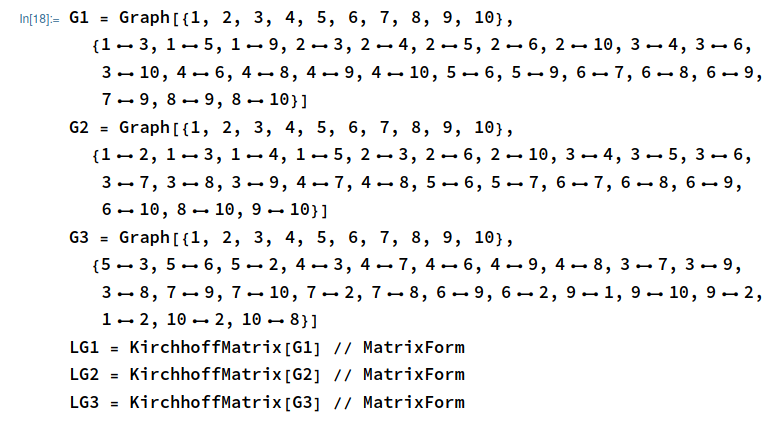
\includegraphics[width=\textwidth]{code_2.png}

The value of graph laplacians is as follows
\begin{align}
    LG1 &=
    \left(
    \begin{array}{cccccccccc}
     3 & 0 & -1 & 0 & -1 & 0 & 0 & 0 & -1 & 0 \\
     0 & 5 & -1 & -1 & -1 & -1 & 0 & 0 & 0 & -1 \\
     -1 & -1 & 5 & -1 & 0 & -1 & 0 & 0 & 0 & -1 \\
     0 & -1 & -1 & 6 & 0 & -1 & 0 & -1 & -1 & -1 \\
     -1 & -1 & 0 & 0 & 4 & -1 & 0 & 0 & -1 & 0 \\
     0 & -1 & -1 & -1 & -1 & 7 & -1 & -1 & -1 & 0 \\
     0 & 0 & 0 & 0 & 0 & -1 & 2 & 0 & -1 & 0 \\
     0 & 0 & 0 & -1 & 0 & -1 & 0 & 4 & -1 & -1 \\
     -1 & 0 & 0 & -1 & -1 & -1 & -1 & -1 & 6 & 0 \\
     0 & -1 & -1 & -1 & 0 & 0 & 0 & -1 & 0 & 4 \\
    \end{array}
    \right) \\
    LG2 &=
    \left(
    \begin{array}{cccccccccc}
     4 & -1 & -1 & -1 & -1 & 0 & 0 & 0 & 0 & 0 \\
     -1 & 4 & -1 & 0 & 0 & -1 & 0 & 0 & 0 & -1 \\
     -1 & -1 & 8 & -1 & -1 & -1 & -1 & -1 & -1 & 0 \\
     -1 & 0 & -1 & 4 & 0 & 0 & -1 & -1 & 0 & 0 \\
     -1 & 0 & -1 & 0 & 4 & -1 & -1 & 0 & 0 & 0 \\
     0 & -1 & -1 & 0 & -1 & 7 & -1 & -1 & -1 & -1 \\
     0 & 0 & -1 & -1 & -1 & -1 & 4 & 0 & 0 & 0 \\
     0 & 0 & -1 & -1 & 0 & -1 & 0 & 4 & 0 & -1 \\
     0 & 0 & -1 & 0 & 0 & -1 & 0 & 0 & 3 & -1 \\
     0 & -1 & 0 & 0 & 0 & -1 & 0 & -1 & -1 & 4 \\
    \end{array}
    \right) \\
    LG3 &=
    \left(
    \begin{array}{cccccccccc}
     2 & -1 & 0 & 0 & 0 & 0 & 0 & 0 & -1 & 0 \\
     -1 & 6 & 0 & 0 & -1 & -1 & -1 & 0 & -1 & -1 \\
     0 & 0 & 5 & -1 & -1 & 0 & -1 & -1 & -1 & 0 \\
     0 & 0 & -1 & 5 & 0 & -1 & -1 & -1 & -1 & 0 \\
     0 & -1 & -1 & 0 & 3 & -1 & 0 & 0 & 0 & 0 \\
     0 & -1 & 0 & -1 & -1 & 4 & 0 & 0 & -1 & 0 \\
     0 & -1 & -1 & -1 & 0 & 0 & 6 & -1 & -1 & -1 \\
     0 & 0 & -1 & -1 & 0 & 0 & -1 & 4 & 0 & -1 \\
     -1 & -1 & -1 & -1 & 0 & -1 & -1 & 0 & 7 & -1 \\
     0 & -1 & 0 & 0 & 0 & 0 & -1 & -1 & -1 & 4 \\
    \end{array}
    \right)
\end{align}

% Start problem 3
\newpage
\subsection*{Problem 3}
\textit{
    Find eigenvalues and show graphs are isomorphic.
}

\solution
Code to generate eigenvalues is shown below (in Python)
\begin{lstlisting}[language=python]
import numpy as np
np.set_printoptions(precision=3, suppress=True)

def get_eigen(m):
    val, vec = np.linalg.eig(m)
    
    idx = val.argsort()
    eigen_val = val[idx]
    eigen_vec = vec[:, idx]
    
    return eigen_val, eigen_vec
    
val1, vec1 = get_eigen(lg1)
val2, vec2 = get_eigen(lg2)
val3, vec3 = get_eigen(lg3)
\end{lstlisting}

The eigenvalues (represented by $val\{i\}$) are as follows
\begin{align*}
    val1 &= 
    \begin{bmatrix}
        0.& 1.78 & 2.318& 3.769& 3.923& 5.221& 6.476& 6.494& 7.702& 8.317
    \end{bmatrix} \\
    val2 &= 
    \begin{bmatrix}
        0.& 2.114& 3.198& 3.204& 3.915& 4.555& 5.477& 6.247& 8.158& 9.131
    \end{bmatrix} \\
    val3 &= 
    \begin{bmatrix}
        0.& 1.78 & 2.318& 3.769& 3.923& 5.221& 6.476& 6.494& 7.702& 8.317
    \end{bmatrix}
\end{align*}

Check for isomorphism
\begin{itemize}
    \item Between $G_1$ and $G_2$ - Not possible as the set of eigenvalues are different
    \item Between $G_2$ and $G_3$ - Not possible as the set of eigenvalues are different
    \item Between $G_3$ and $G_1$ - Possible to find an isomorphism as they have the same set of eigenvalues
\end{itemize}

% Start problem 3
\newpage
\subsection*{Problem 4 (1)}
\textit{
    Find eigenvectors of graphs you found isomorphic
}

\solution
The eigenvectors (represented by $vec\{i\}$) for LG1 and LG3 are as follows
\begin{align*}
    vec1 &= 
    \begin{bmatrix}
        0.316& -0.093& -0.715&  0.085& -0.513&  0.085& -0.267&  0.048& 0.12 &  0.115 \\
        0.316& -0.192&  0.097& -0.412&  0.304& -0.111& -0.71 &  0.099& -0.204& -0.154 \\
        0.316& -0.204&  0.01 & -0.378& -0.264& -0.426&  0.408& -0.452& -0.147& -0.267 \\
        0.316& -0.143&  0.207&  0.029& -0.006& -0.3  &  0.142&  0.527& 0.661& -0.104 \\
        0.316& -0.041& -0.394&  0.009&  0.667&  0.331&  0.265& -0.224& 0.217& -0.146 \\
        0.316&  0.062&  0.059&  0.026&  0.189& -0.284&  0.065& -0.096& -0.085&  0.869 \\
        0.316&  0.879&  0.139& -0.186& -0.135&  0.117& -0.072& -0.091& 0.126& -0.106 \\
        0.316& -0.108&  0.322&  0.717& -0.054& -0.022& -0.255& -0.415& 0.042& -0.168 \\
        0.316&  0.132& -0.104&  0.304&  0.071& -0.093&  0.256&  0.507& -0.636& -0.198 \\
        0.316& -0.291&  0.378& -0.192& -0.259&  0.704&  0.168&  0.096& -0.095&  0.161 \\
    \end{bmatrix} \\
    vec2 &=
    \begin{bmatrix}
        0.316&  0.879& -0.139& -0.186&  0.135& -0.117&  0.072&  0.091& 0.126& -0.106\\
        0.316&  0.132&  0.104&  0.304& -0.071&  0.093& -0.256& -0.507& -0.636& -0.198\\
        0.316& -0.204& -0.01 & -0.378&  0.264&  0.426& -0.408&  0.452& -0.147& -0.267\\
        0.316& -0.192& -0.097& -0.412& -0.304&  0.111&  0.71 & -0.099& -0.204& -0.154\\
        0.316& -0.093&  0.715&  0.085&  0.513& -0.085&  0.267& -0.048& 0.12 &  0.115\\
        0.316& -0.041&  0.394&  0.009& -0.667& -0.331& -0.265&  0.224& 0.217& -0.146\\
        0.316& -0.143& -0.207&  0.029&  0.006&  0.3  & -0.142& -0.527& 0.661& -0.104\\
        0.316& -0.291& -0.378& -0.192&  0.259& -0.704& -0.168& -0.096& -0.095&  0.161\\
        0.316&  0.062& -0.059&  0.026& -0.189&  0.284& -0.065&  0.096& -0.085&  0.869\\
        0.316& -0.108& -0.322&  0.717&  0.054&  0.022&  0.255&  0.415& 0.042& -0.168 \\
    \end{bmatrix}
\end{align*}

\newpage
\subsection*{Problem 4 (2)}
\textit{
    Find a mapping for isomorphism
}

\solution
Using the second eigenvector (i.e. column 2 of above matrices), we can find the mapping from node indexes in $LG1$ and $LG3$. I have written a simple numpy program that can do this for me. But this can also be done manually by just comparing each value of the column to find the corresponding indexes.

Code to get the mapping is as follows:
\begin{lstlisting}[language=python]
col_vec1 = vec1[:, 1]
col_vec3 = vec3[:, 1]
mapping = []

for i in range(vec1.shape[0]):
    exists = False
    for j in range(vec3.shape[0]):
        if np.isclose(col_vec1[i], col_vec3[j]):
            mapping.append([i+1, j+1])
            exists = True
            break
    if not exists:
            print(f'Could not find value')
\end{lstlisting}

The output mapping is as follows:
\begin{align}
    \begin{matrix}
        1 \rightarrow 5 \\
        2 \rightarrow 4 \\
        3 \rightarrow 3 \\
        4 \rightarrow 7 \\
        5 \rightarrow 6 \\
        6 \rightarrow 9 \\
        7 \rightarrow 1 \\
        8 \rightarrow 10 \\
        9 \rightarrow 2 \\
        10 \rightarrow 8 \\
    \end{matrix}
\end{align}

Consider $1 \rightarrow 5$. It means the node at index 1 in $G1$ is at index 5 in $G3$.

$f: \{1,2,3,4,5,6,7,8,9,10\} \rightarrow \{5,4,3,7,6,9,1,10,2,8\}$ is an isomorphism mapping between $G1$ and $G3$.

\newpage
\subsection*{Problem 4 (3)}
\textit{
    Verify edge set under isomorphism
}

\solution
Computing the $f$ for the edge set of $G1$,
\begin{alignat*}{2}
    1 - 3  &\rightarrow f(1) - f(3)  &= 5 - 3  \\
    1 - 5  &\rightarrow f(1) - f(5)  &= 5 - 6  \\
    1 - 9  &\rightarrow f(1) - f(9)  &= 5 - 2  \\
    2 - 3  &\rightarrow f(2) - f(3)  &= 4 - 3  \\
    2 - 4  &\rightarrow f(2) - f(4)  &= 4 - 7  \\
    2 - 5  &\rightarrow f(2) - f(5)  &= 4 - 6  \\
    2 - 6  &\rightarrow f(2) - f(6)  &= 4 - 9  \\
    2 - 10 &\rightarrow f(2) - f(10) &= 4 - 8  \\
    3 - 4  &\rightarrow f(3) - f(4)  &= 3 - 7  \\
    3 - 6  &\rightarrow f(3) - f(6)  &= 3 - 9  \\
    3 - 10 &\rightarrow f(3) - f(10) &= 3 - 8  \\
    4 - 6  &\rightarrow f(4) - f(6)  &= 7 - 9  \\
    4 - 8  &\rightarrow f(4) - f(8)  &= 7 - 10 \\ 
    4 - 9  &\rightarrow f(4) - f(9)  &= 7 - 2  \\
    4 - 10 &\rightarrow f(4) - f(10) &= 7 - 8  \\
    5 - 6  &\rightarrow f(5) - f(6)  &= 6 - 9  \\
    5 - 9  &\rightarrow f(5) - f(9)  &= 6 - 2  \\
    6 - 7  &\rightarrow f(6) - f(7)  &= 9 - 1  \\
    6 - 8  &\rightarrow f(6) - f(8)  &= 9 - 10 \\ 
    6 - 9  &\rightarrow f(6) - f(9)  &= 9 - 2  \\
    7 - 9  &\rightarrow f(7) - f(9)  &= 1 - 2  \\
    8 - 9  &\rightarrow f(8) - f(9)  &= 10 - 2 \\ 
    8 - 10 &\rightarrow f(8) - f(1)  &= 10 - 8 \\
\end{alignat*}

Column 3 of above is same as the edge set of $G3$. Thus we verified the the proposed isomorphism in 4(2) is correct.

\newpage
\subsection*{Problem 5}
\textit{
    Draw graphs
}

\solution
The code to generate the drawings is shown below
\begin{lstlisting}[language=python]
import networkx as nx
import matplotlib.pyplot as plt

def draw_graph(graph, title):
    G = nx.Graph()
    
    for i in range(1, 11): G.add_node(i)
    for edge in graph    : G.add_edge(edge[0], edge[1])
    
    pos = nx.spectral_layout(G)
    nx.draw(G, pos, with_labels=True, node_size=200)
    plt.savefig(f"{title}.png")
    
draw_graph(G1, "G1")
draw_graph(G2, "G2")
draw_graph(G3, "G3")
\end{lstlisting}

\begin{figure}[H]
    \begin{tabular}{c}
    \subfloat[\text{Graph G1}]{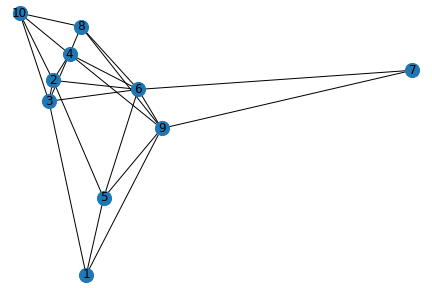
\includegraphics[width=11cm]{G1.png}} \\
    \subfloat["Graph G2"]{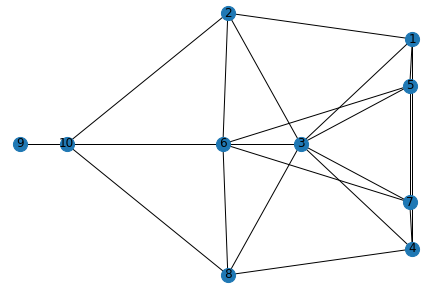
\includegraphics[width=11cm]{G2.png}} \\
    \subfloat["Graph G3"]{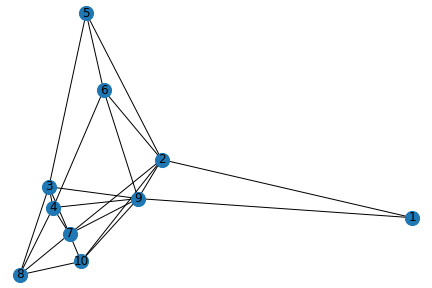
\includegraphics[width=11cm]{G3.png}} \\
    \end{tabular}
\end{figure}
\end{document}
